\section{tasks::testtask Class Reference}
\label{classtasks_1_1testtask}\index{tasks::testtask@{tasks::testtask}}
Inheritance diagram for tasks::testtask::\begin{figure}[H]
\begin{center}
\leavevmode
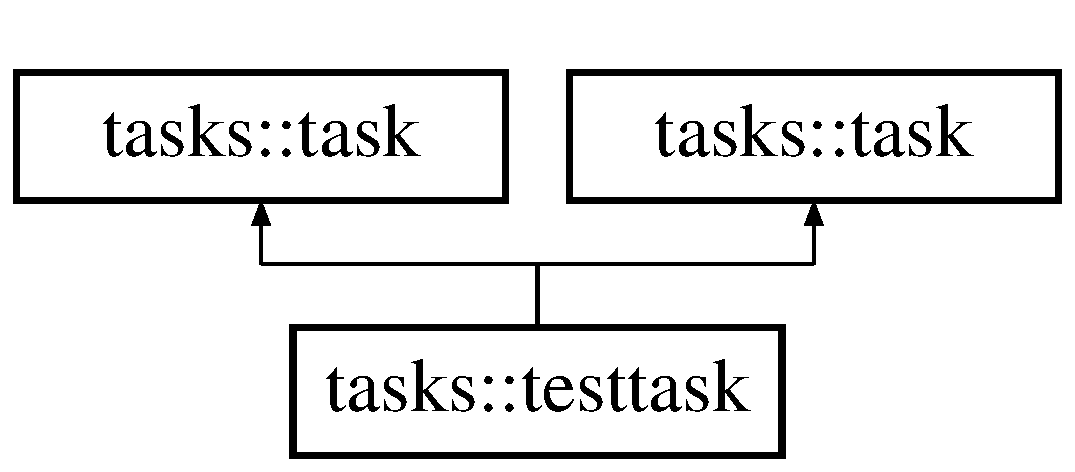
\includegraphics[height=2cm]{classtasks_1_1testtask}
\end{center}
\end{figure}
\subsection*{Public Member Functions}
\begin{CompactItemize}
\item 
def \textbf{run}\label{classtasks_1_1testtask_00fe50b803e43fde0d25bfc73aa436c1}

\item 
def \textbf{run}\label{classtasks_1_1testtask_00fe50b803e43fde0d25bfc73aa436c1}

\end{CompactItemize}
\subsection*{Static Public Attributes}
\begin{CompactItemize}
\item 
string \textbf{name} = 'skeleton'\label{classtasks_1_1testtask_8f077e1e4f67469fa5cf6e0c22a02997}

\item 
string \textbf{button\-Text} = 'Does really nothing!'\label{classtasks_1_1testtask_53905d7258165161f7a752124a7e4aba}

\end{CompactItemize}


\subsection{Detailed Description}


\footnotesize\begin{verbatim}
   This task does nothing (except for writing to the log file). The help text
   that should appear in the interface should go here
\end{verbatim}
\normalsize
 



The documentation for this class was generated from the following files:\begin{CompactItemize}
\item 
old/PANICtool-1.0/tasks.py\item 
old/tasks.py\end{CompactItemize}
